\documentclass[11pt]{article}

% === Packages ===
\usepackage[margin=1in]{geometry}
\usepackage{amsmath,amssymb,amsfonts}
\usepackage{graphicx}
\usepackage{booktabs}
\usepackage{multirow}
\usepackage{hyperref}
\usepackage{xcolor}
\usepackage{enumitem}
\usepackage{caption}
\usepackage{subcaption}
\usepackage{array}
\usepackage{algorithm}
\usepackage{algpseudocode}
\usepackage{bm}
\usepackage{tikz}
\usetikzlibrary{positioning,arrows.meta,fit,calc,decorations.pathreplacing}

% === Custom Commands ===
\newcommand{\RR}{\mathbb{R}}
\newcommand{\layernorm}{\text{LayerNorm}}
\newcommand{\softmax}{\text{softmax}}
\newcommand{\gelu}{\text{GELU}}
\newcommand{\concat}{\text{Concat}}
\newcommand{\attn}{\text{Attention}}
\newcommand{\ffn}{\text{FFN}}
\newcommand{\moe}{\text{MoE}}
\newcommand{\lacuna}{\textsc{Lacuna}}

\title{\lacuna{}: A BERT-Inspired Transformer Architecture \\
for Missing Data Mechanism Classification}
\author{Progress Report --- Architecture Specification}
\date{\today}

\begin{document}
\maketitle

\begin{abstract}
We describe the architecture of \lacuna{}, a transformer-based classifier that determines the missing data mechanism (MCAR, MAR, or MNAR) operating on a given tabular dataset. \lacuna{} inherits core design principles from BERT~\cite{devlin2019bert}---bidirectional self-attention, pre-norm transformer layers, and masked prediction as a pretraining signal---but introduces fundamental modifications for the tabular missing-data domain: four-dimensional cell tokens, row-wise attention scope, hierarchical two-stage attention pooling, mechanism-specific reconstruction heads, explicit statistical missingness features, and a Mixture-of-Experts gating network that produces calibrated posterior probabilities over the three mechanism classes. The base configuration uses 4 transformer layers, 4 attention heads, hidden dimension 128, and achieves 82.6\% classification accuracy with 901,130 parameters.
\end{abstract}

% =====================================================================
\section{Introduction and Relationship to BERT}
% =====================================================================

BERT (Bidirectional Encoder Representations from Transformers)~\cite{devlin2019bert} demonstrated that bidirectional self-attention over masked sequences produces powerful contextual representations for natural language understanding. \lacuna{} adapts this insight to a fundamentally different domain: tabular datasets with missing values. The core analogy is:

\begin{center}
\begin{tabular}{lll}
\toprule
\textbf{Concept} & \textbf{BERT} & \textbf{\lacuna{}} \\
\midrule
Input unit & Word token & Table cell (4D token) \\
Sequence & Sentence & Row of features \\
Masking & Random word masking & Natural + artificial cell masking \\
Prediction task & Predict masked word & Predict masked cell value \\
Classification task & Sentence-pair (NLI) & Mechanism class (MCAR/MAR/MNAR) \\
Sequence repr. & {[CLS]} token & Hierarchical attention pooling \\
Layers / Heads & 12 / 12 (BERT-Base) & 4 / 4 (\lacuna{}-Base) \\
Hidden dim & 768 & 128 \\
Parameters & 110M & 901K \\
\bottomrule
\end{tabular}
\end{center}

The key insight enabling this transfer is that \emph{MAR manifests as cross-column dependencies within rows}---precisely the kind of contextual relationship that self-attention excels at capturing. Under MAR, the probability of a value being missing in column $j$ depends on observed values in other columns within the same row: $P(R_{ij} = 1 \mid X_{\text{obs}}) \neq P(R_{ij} = 1)$, where $R_{ij}$ is the missingness indicator. Self-attention over features within a row can learn these dependencies, just as BERT's self-attention learns word-to-word dependencies within a sentence.

% =====================================================================
\section{Input Representation}
\label{sec:input}
% =====================================================================

\subsection{Token Structure}

Unlike BERT, which maps discrete word tokens to dense vectors via vocabulary lookup, \lacuna{} operates on continuous-valued table cells. Each cell in the dataset is represented as a 4-dimensional token:

\begin{equation}
\mathbf{t}_{ij} = \begin{bmatrix} v_{ij} \\ o_{ij} \\ m_{ij} \\ p_j \end{bmatrix} \in \RR^4
\label{eq:token}
\end{equation}

where:
\begin{itemize}[nosep]
    \item $v_{ij} \in \RR$: Robust-normalized value (approximately in $[-3, 3]$), set to 0 if missing.
    \item $o_{ij} \in \{0, 1\}$: Observation indicator (1 = observed, 0 = missing).
    \item $m_{ij} \in \{0, 1\}$: Mask type (0 = naturally missing, 1 = artificially masked for self-supervised pretraining).
    \item $p_j = j / (\text{max\_cols} - 1) \in [0, 1]$: Normalized feature position.
\end{itemize}

The input to the model is a tensor of shape $[B, n, d, 4]$, where $B$ is the batch size, $n \leq 128$ is the number of rows, and $d \leq 48$ is the number of features (columns). Both $n$ and $d$ are padded to maximum values with corresponding boolean masks $\mathbf{M}_{\text{row}} \in \{0,1\}^{B \times n}$ and $\mathbf{M}_{\text{col}} \in \{0,1\}^{B \times d}$.

\paragraph{Comparison to BERT.} BERT's input is a sequence of discrete token IDs mapped to dense vectors through a learned vocabulary embedding. \lacuna{} instead receives continuous-valued cells with explicit binary indicators for observation status and mask type. This separation is critical: it enables the model to independently learn patterns like ``high values go missing'' (MNAR signal in $v_{ij}$ conditioned on $o_{ij} = 0$) versus ``missingness is uniform regardless of value'' (MCAR signal).

% =====================================================================
\section{Token Embedding Layer}
\label{sec:embedding}
% =====================================================================

The 4D token $\mathbf{t}_{ij}$ is projected to the hidden dimension $h = 128$ through four parallel embedding pathways, each producing a vector of dimension $h/4 = 32$:

\begin{align}
\mathbf{e}^{\text{val}}_{ij} &= \text{Linear}_{1 \to 32}\!\left(v_{ij} \cdot o_{ij}\right) \in \RR^{32} \label{eq:val_emb} \\
\mathbf{e}^{\text{obs}}_{ij} &= \text{Embed}_{\{0,1\} \to 32}\!\left(o_{ij}\right) \in \RR^{32} \label{eq:obs_emb} \\
\mathbf{e}^{\text{mask}}_{ij} &= \text{Embed}_{\{0,1\} \to 32}\!\left(m_{ij}\right) \in \RR^{32} \label{eq:mask_emb} \\
\mathbf{e}^{\text{pos}}_{ij} &= \text{Embed}_{\{0,\ldots,31\} \to 32}\!\left(\lfloor p_j \cdot 31 \rfloor\right) \in \RR^{32} \label{eq:pos_emb}
\end{align}

Note that in Equation~\eqref{eq:val_emb}, the raw value $v_{ij}$ is scaled by the observation indicator $o_{ij}$, so missing cells contribute zero to the value embedding. This prevents the model from leaking information about placeholder values.

The four components are concatenated and projected:
\begin{equation}
\mathbf{h}^{(0)}_{ij} = \text{Dropout}_{0.1}\!\left(\layernorm\!\left(\text{Linear}_{128 \to 128}\!\left([\mathbf{e}^{\text{val}}_{ij}; \mathbf{e}^{\text{obs}}_{ij}; \mathbf{e}^{\text{mask}}_{ij}; \mathbf{e}^{\text{pos}}_{ij}]\right)\right)\right) \in \RR^{128}
\label{eq:token_embed}
\end{equation}

\paragraph{Comparison to BERT.} BERT sums three embeddings (token + position + segment). \lacuna{} concatenates four embeddings and projects, because the four token components carry orthogonal information that should not be mixed before the projection. BERT uses segment embeddings for sentence-pair tasks; \lacuna{} replaces these with mask-type embeddings that distinguish natural missingness from artificial masking.

% =====================================================================
\section{Transformer Encoder}
\label{sec:encoder}
% =====================================================================

\subsection{Architecture Overview}

The encoder consists of $L = 4$ stacked transformer layers, each applying pre-norm multi-head self-attention followed by a position-wise feedforward network. The output shape is preserved: $[B, n, d, h]$ at every layer.

\begin{table}[h]
\centering
\caption{Encoder hyperparameters for the three model variants.}
\label{tab:encoder_config}
\begin{tabular}{lccc}
\toprule
\textbf{Parameter} & \textbf{Mini} & \textbf{Base} & \textbf{Large} \\
\midrule
Hidden dimension ($h$) & 64 & \textbf{128} & 256 \\
Evidence dimension ($p$) & 32 & \textbf{64} & 128 \\
Transformer layers ($L$) & 2 & \textbf{4} & 6 \\
Attention heads ($H$) & 2 & \textbf{4} & 8 \\
Head dimension ($d_k = h/H$) & 32 & \textbf{32} & 32 \\
FFN inner dimension ($d_{\text{ff}}$) & 256 & \textbf{512} & 1024 \\
Max columns ($d_{\max}$) & 32 & \textbf{32} & 64 \\
Dropout & 0.1 & \textbf{0.1} & 0.1 \\
Row pooling & mean & \textbf{attention} & attention \\
Dataset pooling & mean & \textbf{attention} & attention \\
\bottomrule
\end{tabular}
\end{table}

\subsection{Row-Wise Multi-Head Self-Attention}

A critical departure from BERT: \lacuna{} applies self-attention \emph{within each row independently}, not across the entire input. The input tensor is reshaped from $[B, n, d, h]$ to $[Bn, d, h]$, treating each row as a separate sequence of $d$ feature tokens.

For layer $\ell \in \{1, \ldots, L\}$, the pre-norm attention computation is:

\begin{align}
\hat{\mathbf{H}}^{(\ell)} &= \layernorm\!\left(\mathbf{H}^{(\ell-1)}\right) \label{eq:prenorm_attn} \\
\mathbf{Q} &= \hat{\mathbf{H}}^{(\ell)} \mathbf{W}_Q^{(\ell)}, \quad
\mathbf{K} = \hat{\mathbf{H}}^{(\ell)} \mathbf{W}_K^{(\ell)}, \quad
\mathbf{V} = \hat{\mathbf{H}}^{(\ell)} \mathbf{W}_V^{(\ell)} \label{eq:qkv}
\end{align}

where $\mathbf{W}_Q^{(\ell)}, \mathbf{W}_K^{(\ell)}, \mathbf{W}_V^{(\ell)} \in \RR^{128 \times 128}$ are learned projection matrices. Each is conceptually split into $H = 4$ heads of dimension $d_k = 32$:

\begin{equation}
\mathbf{Q} = [\mathbf{Q}_1; \ldots; \mathbf{Q}_4], \quad
\mathbf{K} = [\mathbf{K}_1; \ldots; \mathbf{K}_4], \quad
\mathbf{V} = [\mathbf{V}_1; \ldots; \mathbf{V}_4]
\end{equation}

where $\mathbf{Q}_i, \mathbf{K}_i, \mathbf{V}_i \in \RR^{d \times 32}$ for each head $i$.

The scaled dot-product attention for each head is:
\begin{equation}
\text{head}_i = \softmax\!\left(\frac{\mathbf{Q}_i \mathbf{K}_i^\top}{\sqrt{d_k}} + \mathbf{M}_{\text{attn}}\right) \mathbf{V}_i \in \RR^{d \times 32}
\label{eq:attention}
\end{equation}

where $d_k = 32$ is the head dimension and $\mathbf{M}_{\text{attn}} \in \RR^{d \times d}$ is an attention mask that sets padding positions to $-\infty$ before the softmax. The attention weight matrix $\mathbf{A}_i = \softmax(\mathbf{Q}_i \mathbf{K}_i^\top / \sqrt{d_k} + \mathbf{M}_{\text{attn}}) \in \RR^{d \times d}$ has entry $(j, k)$ representing how much feature $j$ attends to feature $k$ within the same row.

The heads are concatenated and projected:
\begin{equation}
\text{MHA}(\hat{\mathbf{H}}^{(\ell)}) = [\text{head}_1; \ldots; \text{head}_4] \, \mathbf{W}_O^{(\ell)} \in \RR^{d \times 128}
\label{eq:mha_output}
\end{equation}

where $\mathbf{W}_O^{(\ell)} \in \RR^{128 \times 128}$ is the output projection. The residual connection then yields:

\begin{equation}
\tilde{\mathbf{H}}^{(\ell)} = \mathbf{H}^{(\ell-1)} + \text{Dropout}_{0.1}\!\left(\text{MHA}(\hat{\mathbf{H}}^{(\ell)})\right)
\label{eq:attn_residual}
\end{equation}

\paragraph{Why row-wise, not full-dataset attention?} Under MAR, missingness in column $j$ depends on values in \emph{other columns within the same row}: $P(R_{ij} \mid X_{i, \text{obs}})$. Cross-row attention would capture dataset-level summary statistics (e.g., ``column 1 is 30\% missing'') but not the row-level dependencies that define MAR. Additionally, row-wise attention has $O(d^2)$ memory per row, versus $O(n^2 d^2)$ for full-dataset attention, enabling processing of datasets with hundreds of rows.

\subsection{Position-Wise Feedforward Network}

After attention, each token passes through a two-layer feedforward network with GELU activation:

\begin{align}
\hat{\tilde{\mathbf{H}}}^{(\ell)} &= \layernorm\!\left(\tilde{\mathbf{H}}^{(\ell)}\right) \label{eq:prenorm_ff} \\
\ffn(\hat{\tilde{\mathbf{H}}}^{(\ell)}) &= \text{Linear}_{512 \to 128}\!\left(\text{Dropout}_{0.1}\!\left(\gelu\!\left(\text{Linear}_{128 \to 512}\!\left(\hat{\tilde{\mathbf{H}}}^{(\ell)}\right)\right)\right)\right) \label{eq:ffn}
\end{align}

\begin{equation}
\mathbf{H}^{(\ell)} = \tilde{\mathbf{H}}^{(\ell)} + \text{Dropout}_{0.1}\!\left(\ffn(\hat{\tilde{\mathbf{H}}}^{(\ell)})\right) \in \RR^{d \times 128}
\label{eq:ff_residual}
\end{equation}

The FFN expands the hidden dimension by a factor of 4 (128 $\to$ 512) before projecting back, following standard transformer practice.

\paragraph{Comparison to BERT.} BERT-Base uses the same FFN structure but with dimensions 768 $\to$ 3072 $\to$ 768. Both use pre-norm residual connections, though original BERT used post-norm; \lacuna{} adopts pre-norm for improved training stability with fewer layers. BERT uses GELU activation; \lacuna{} does the same.

% =====================================================================
\section{Hierarchical Attention Pooling}
\label{sec:pooling}
% =====================================================================

After $L = 4$ transformer layers, the output has shape $[B, n, d, 128]$---a representation for every cell in every row. This must be compressed to a single \emph{evidence vector} $\mathbf{z} \in \RR^{64}$ summarizing the entire dataset. \lacuna{} accomplishes this through two-stage hierarchical attention pooling, replacing BERT's [CLS] token approach.

\subsection{Stage 1: Row Pooling (Features $\to$ Rows)}

For each row $i$, the $d$ feature representations $\{\mathbf{h}^{(L)}_{i1}, \ldots, \mathbf{h}^{(L)}_{id}\}$ are aggregated into a single row vector via learned attention:

\begin{align}
\alpha_{ij} &= \frac{\exp\!\left(s(\mathbf{h}^{(L)}_{ij})\right)}{\sum_{k=1}^{d} \exp\!\left(s(\mathbf{h}^{(L)}_{ik})\right) \cdot [\mathbf{M}_{\text{col}}]_k} \label{eq:row_pool_weights} \\
\mathbf{r}_i &= \sum_{j=1}^{d} \alpha_{ij} \cdot \mathbf{h}^{(L)}_{ij} \in \RR^{128} \label{eq:row_pool}
\end{align}

where $s: \RR^{128} \to \RR$ is a learned scoring function:
\begin{equation}
s(\mathbf{x}) = \text{Linear}_{64 \to 1}\!\left(\tanh\!\left(\text{Linear}_{128 \to 64}(\mathbf{x})\right)\right)
\label{eq:attn_scorer}
\end{equation}

This transforms the tensor from $[B, n, d, 128]$ to $[B, n, 128]$.

\subsection{Stage 2: Dataset Pooling (Rows $\to$ Dataset)}

The $n$ row representations $\{\mathbf{r}_1, \ldots, \mathbf{r}_n\}$ are aggregated identically into a single dataset vector:

\begin{align}
\beta_i &= \frac{\exp\!\left(s'(\mathbf{r}_i)\right)}{\sum_{k=1}^{n} \exp\!\left(s'(\mathbf{r}_k)\right) \cdot [\mathbf{M}_{\text{row}}]_k} \label{eq:dataset_pool_weights} \\
\mathbf{z} &= \layernorm\!\left(\text{Linear}_{128 \to 64}\!\left(\layernorm\!\left(\sum_{i=1}^{n} \beta_i \cdot \mathbf{r}_i\right)\right)\right) \in \RR^{64} \label{eq:evidence}
\end{align}

where $s'$ has the same architecture as $s$ (Equation~\ref{eq:attn_scorer}) but with separate parameters.

\paragraph{Why not a [CLS] token?} Tabular data has no privileged ``start of sequence'' position. A [CLS] token prepended to each row would need to learn to attend to the most informative features without positional bias. The learned attention pooling explicitly computes importance weights, allowing the model to learn that, e.g., ``rows with partial missingness are most informative for MAR detection'' and ``features with extreme values matter most for MNAR detection.''

% =====================================================================
\section{Reconstruction Heads}
\label{sec:reconstruction}
% =====================================================================

Before classification, \lacuna{} employs a set of $K = 3$ reconstruction heads (in the default 1/1/1 symmetric configuration) that attempt to predict the values of missing cells. These serve a dual purpose: (1) as a self-supervised pretraining signal and (2) as a \emph{discrimination signal}---the pattern of reconstruction errors across the different heads reveals the underlying mechanism.

Each head receives the token-level representations $\mathbf{H}^{(L)} \in \RR^{B \times n \times d \times 128}$ and produces per-cell value predictions. The heads differ in their architectural inductive biases:

\subsection{MCAR Head}

A simple MLP applied independently to each token:
\begin{equation}
\hat{v}^{\text{MCAR}}_{ij} = \text{Linear}_{64 \to 1}\!\left(\gelu\!\left(\layernorm\!\left(\text{Linear}_{128 \to 64}\!\left(\mathbf{h}^{(L)}_{ij}\right)\right)\right)\right)
\label{eq:mcar_head}
\end{equation}

This head exploits no cross-column structure and can only use global distributional information encoded in each token's representation.

\subsection{MAR Head (Cross-Attention to Raw Observed Values)}

The MAR head uses a cross-attention mechanism where queries and keys are derived from the learned representations, but the \emph{values} are the raw observed data:

\begin{align}
\mathbf{Q}^{\text{mar}} &= \mathbf{H}^{(L)} \mathbf{W}^{\text{mar}}_Q \in \RR^{d \times 64} \label{eq:mar_q} \\
\mathbf{K}^{\text{mar}} &= \mathbf{H}^{(L)} \mathbf{W}^{\text{mar}}_K \in \RR^{d \times 64} \label{eq:mar_k} \\
\mathbf{V}^{\text{mar}} &= \text{Linear}_{1 \to 64}\!\left(\mathbf{X}_{\text{raw}}\right) \in \RR^{d \times 64} \label{eq:mar_v}
\end{align}

where $\mathbf{X}_{\text{raw}} \in \RR^{d \times 1}$ contains the raw observed values ($v_{ij}$ from the input tokens). Attention is masked to attend \emph{only to observed cells}:

\begin{equation}
\mathbf{C}_{ij} = \softmax\!\left(\frac{\mathbf{Q}^{\text{mar}}_j (\mathbf{K}^{\text{mar}})^\top}{\sqrt{64}} + \mathbf{M}_{\text{obs}}\right) \mathbf{V}^{\text{mar}} \in \RR^{64}
\label{eq:mar_attn}
\end{equation}

where $[\mathbf{M}_{\text{obs}}]_{jk} = -\infty$ if cell $k$ is unobserved, and 0 otherwise. The context $\mathbf{C}_{ij}$ is then concatenated with the original representation and passed through a predictor MLP:

\begin{equation}
\hat{v}^{\text{MAR}}_{ij} = \text{MLP}_{192 \to 64 \to 1}\!\left([\mathbf{C}_{ij}; \mathbf{h}^{(L)}_{ij}]\right)
\label{eq:mar_pred}
\end{equation}

Under MAR, this head should achieve \emph{lower} reconstruction error than the MCAR head on naturally missing cells, because the cross-attention can learn to use observed values in correlated columns to predict missing ones. Under MNAR, both heads perform similarly because the missing value depends on itself, not on other columns.

\subsection{MNAR Self-Censoring Head}

This head models the hypothesis that extreme values are systematically censored:
\begin{align}
\hat{v}^{\text{base}}_{ij} &= \text{MLP}_{128 \to 64 \to 1}\!\left(\mathbf{h}^{(L)}_{ij}\right) \label{eq:mnar_base} \\
c_{ij} &= \gamma \cdot \tanh\!\left(\text{MLP}_{128 \to 64 \to 1}\!\left(\mathbf{h}^{(L)}_{ij}\right)\right) \label{eq:mnar_censor} \\
\hat{v}^{\text{MNAR}}_{ij} &= \hat{v}^{\text{base}}_{ij} + c_{ij} \cdot (1 - o_{ij}) \label{eq:mnar_pred}
\end{align}

where $\gamma$ is a learnable censoring scale parameter. The censoring adjustment $c_{ij}$ is only applied to missing cells ($o_{ij} = 0$), learning whether missing values tend to be higher or lower than the population mean.

\subsection{Discrimination Signal}

The key insight: reconstruction errors on \emph{naturally missing} cells (not artificially masked) differ across heads depending on the true mechanism:

\begin{center}
\begin{tabular}{lccc}
\toprule
\textbf{True Mechanism} & $\epsilon_{\text{MCAR}}$ & $\epsilon_{\text{MAR}}$ & $\epsilon_{\text{MNAR}}$ \\
\midrule
MCAR & Moderate & Moderate & Moderate \\
MAR & Higher & \textbf{Lower} & Higher \\
MNAR & Variable & Higher & \textbf{Lower} \\
\bottomrule
\end{tabular}
\end{center}

The error vector $\bm{\epsilon} = [\epsilon_{\text{MCAR}}, \epsilon_{\text{MAR}}, \epsilon_{\text{MNAR}}] \in \RR^3$ is passed to the gating network as a discrimination signal.

% =====================================================================
\section{Missingness Feature Extractor}
\label{sec:missingness_features}
% =====================================================================

While reconstruction errors discriminate MAR from MNAR, they are insufficient for MCAR vs.\ MAR discrimination (the cross-attention improves prediction under both, with a small gap). To address this, \lacuna{} computes 16 explicit statistical features from the raw data, organized into five groups:

\begin{table}[h]
\centering
\caption{Missingness pattern features (16 total, non-learnable).}
\label{tab:miss_features}
\begin{tabular}{llcl}
\toprule
\textbf{Group} & \textbf{Features} & \textbf{Count} & \textbf{Primary Signal} \\
\midrule
Missing rate statistics & mean, var, range, max of per-col rates & 4 & MCAR vs MAR \\
Point-biserial corr. & mean, max, std of $\text{corr}(R_j, X_k)$ & 3 & MCAR vs MAR \\
Cross-col miss.\ corr. & mean, max cross-corr, frac.\ high & 3 & MCAR vs MAR \\
Distributional stats & mean skew, mean kurt, var of each & 4 & MAR vs MNAR \\
Little's MCAR approx. & chi-sq statistic, significance proxy & 2 & MCAR vs non-MCAR \\
\bottomrule
\end{tabular}
\end{table}

The missing rate variance alone achieves Cohen's $d > 9.0$ between MCAR and MAR (MCAR produces nearly uniform per-column missing rates; MAR produces highly variable rates). These features require no learned parameters.

The feature vector $\mathbf{f} \in \RR^{16}$ is concatenated with the evidence vector and reconstruction errors as input to the gating network.

% =====================================================================
\section{Mixture of Experts and Classification}
\label{sec:moe}
% =====================================================================

\subsection{Gating Network}

The Mixture of Experts (MoE) layer receives three concatenated input signals:

\begin{equation}
\mathbf{g}_{\text{input}} = [\mathbf{z}; \bm{\epsilon}; \mathbf{f}] \in \RR^{83}
\label{eq:gate_input}
\end{equation}

where $\mathbf{z} \in \RR^{64}$ is the evidence vector (Section~\ref{sec:pooling}), $\bm{\epsilon} \in \RR^{3}$ is the reconstruction error vector (Section~\ref{sec:reconstruction}), and $\mathbf{f} \in \RR^{16}$ is the missingness feature vector (Section~\ref{sec:missingness_features}).

The gating network is a 2-layer MLP producing logits over $K = 3$ experts:

\begin{align}
\mathbf{u} &= \text{Dropout}_{0.1}\!\left(\gelu\!\left(\layernorm\!\left(\text{Linear}_{83 \to 64}(\mathbf{g}_{\text{input}})\right)\right)\right) \in \RR^{64} \label{eq:gate_hidden} \\
\bm{\ell} &= \text{Linear}_{64 \to 3}(\mathbf{u}) \in \RR^{3} \label{eq:gate_logits}
\end{align}

\subsection{Temperature-Scaled Softmax}

Expert probabilities are obtained via temperature-scaled softmax:
\begin{equation}
\pi_k = \frac{\exp(\ell_k / T)}{\sum_{k'=1}^{3} \exp(\ell_{k'} / T)}, \quad k \in \{\text{MCAR}, \text{MAR}, \text{MNAR}\}
\label{eq:temp_softmax}
\end{equation}

The temperature $T$ is set post-hoc to $T = 1.96$ based on calibration on a held-out validation set. This calibration unexpectedly improved both expected calibration error (ECE = 0.038) \emph{and} classification accuracy, by softening overconfident wrong predictions.

\subsection{Expert-to-Class Mapping}

In the default 1/1/1 symmetric configuration (one expert per mechanism class), the expert probabilities map directly to class posteriors:
\begin{equation}
P(\text{class} = c \mid \mathcal{D}) = \pi_c, \quad c \in \{0, 1, 2\}
\label{eq:class_posterior}
\end{equation}

With the balanced ``mean'' aggregation, the posteriors are normalized by the number of experts per class to prevent structural bias (this matters when using $>1$ MNAR variant).

\subsection{Bayes-Optimal Decision Rule}

Given the posterior $\mathbf{p} = [P(\text{MCAR}), P(\text{MAR}), P(\text{MNAR})]$, the model selects an action $a^* \in \{\text{Green}, \text{Yellow}, \text{Red}\}$ that minimizes expected loss:

\begin{equation}
a^* = \arg\min_{a} \sum_{c \in \{0,1,2\}} P(c \mid \mathcal{D}) \cdot L[a, c]
\label{eq:bayes_decision}
\end{equation}

The loss matrix $\mathbf{L} \in \RR^{3 \times 3}$ encodes the cost of choosing action $a$ when the true mechanism is $c$:

\begin{equation}
\mathbf{L} = \begin{bmatrix}
0.0 & 0.3 & 1.0 \\
0.2 & 0.0 & 0.2 \\
1.0 & 0.3 & 0.0
\end{bmatrix}
\quad
\begin{array}{l}
\text{Row 0: Green (assume MCAR)} \\
\text{Row 1: Yellow (assume MAR)} \\
\text{Row 2: Red (assume MNAR)}
\end{array}
\label{eq:loss_matrix}
\end{equation}

The matrix is asymmetric: treating MNAR data as MCAR (top-right, $L = 1.0$) is the costliest error, while the Yellow action (MAR assumption) is the safest default with moderate cost under both MCAR and MNAR.

% =====================================================================
\section{Training}
\label{sec:training}
% =====================================================================

\subsection{Multi-Task Loss}

The total training loss combines classification and reconstruction objectives:
\begin{equation}
\mathcal{L} = \lambda_{\text{cls}} \cdot \mathcal{L}_{\text{cls}} + \lambda_{\text{recon}} \cdot \mathcal{L}_{\text{recon}} + \mathcal{L}_{\text{aux}}
\label{eq:total_loss}
\end{equation}

where:
\begin{itemize}[nosep]
    \item $\mathcal{L}_{\text{cls}}$: Cross-entropy loss on mechanism class posterior vs.\ ground-truth label ($\lambda_{\text{cls}} = 1.0$).
    \item $\mathcal{L}_{\text{recon}}$: MSE on artificially-masked cell predictions, averaged over all heads ($\lambda_{\text{recon}} = 0.5$).
    \item $\mathcal{L}_{\text{aux}}$: Auxiliary losses (load balancing, entropy regularization, KL divergence for the MNAR latent head).
\end{itemize}

\subsection{Training Configuration}

\begin{table}[h]
\centering
\caption{Production training configuration.}
\label{tab:training}
\begin{tabular}{lr}
\toprule
\textbf{Parameter} & \textbf{Value} \\
\midrule
Epochs & 100 \\
Batch size & 16 \\
Batches per epoch & 200 \\
Learning rate & $3 \times 10^{-4}$ \\
Optimizer & AdamW ($\beta_1 = 0.9$, $\beta_2 = 0.999$) \\
Weight decay & 0.01 \\
Gradient clipping & 1.0 \\
Warmup steps & 400 \\
Early stopping patience & 20 epochs \\
Training datasets & 24 (UCI/OpenML) \\
Validation datasets & 7 \\
Missingness generators & 110 total (32 MCAR, $\sim$36 MAR, $\sim$42 MNAR) \\
Total parameters & 901,130 \\
Post-hoc temperature & $T = 1.96$ \\
\bottomrule
\end{tabular}
\end{table}

% =====================================================================
\section{Complete Forward Pass}
\label{sec:forward}
% =====================================================================

Algorithm~\ref{alg:forward} summarizes the complete forward pass with tensor shapes.

\begin{algorithm}[h]
\caption{\lacuna{} Forward Pass (Base Configuration)}
\label{alg:forward}
\begin{algorithmic}[1]
\Require Token batch $\mathbf{T} \in \RR^{B \times 128 \times 48 \times 4}$, masks $\mathbf{M}_{\text{row}}, \mathbf{M}_{\text{col}}$
\Ensure Posterior $\mathbf{p} \in [0,1]^{B \times 3}$, decision $a \in \{0,1,2\}^B$
\State \textbf{Token Embedding:} $\mathbf{H}^{(0)} \gets \text{TokenEmbed}(\mathbf{T}) \in \RR^{B \times 128 \times 48 \times 128}$
\For{$\ell = 1$ to $4$}
    \State \textbf{Self-Attention:} $\tilde{\mathbf{H}}^{(\ell)} \gets \mathbf{H}^{(\ell-1)} + \text{MHA}(\layernorm(\mathbf{H}^{(\ell-1)}))$
    \State \textbf{FFN:} $\mathbf{H}^{(\ell)} \gets \tilde{\mathbf{H}}^{(\ell)} + \ffn(\layernorm(\tilde{\mathbf{H}}^{(\ell)}))$
\EndFor
\State \textbf{Row Pooling:} $\mathbf{R} \gets \text{AttnPool}_{\text{col}}(\mathbf{H}^{(4)}) \in \RR^{B \times 128 \times 128}$
\State \textbf{Dataset Pooling:} $\mathbf{z} \gets \layernorm(\text{Linear}_{128 \to 64}(\text{AttnPool}_{\text{row}}(\mathbf{R}))) \in \RR^{B \times 64}$
\State \textbf{Reconstruction:} $\bm{\epsilon} \gets \text{ReconHeads}(\mathbf{H}^{(4)}, \mathbf{T}) \in \RR^{B \times 3}$
\State \textbf{Miss.\ Features:} $\mathbf{f} \gets \text{StatFeatures}(\mathbf{T}) \in \RR^{B \times 16}$
\State \textbf{Gating:} $\bm{\ell} \gets \text{GateMLP}([\mathbf{z}; \bm{\epsilon}; \mathbf{f}]) \in \RR^{B \times 3}$
\State \textbf{Posterior:} $\mathbf{p} \gets \softmax(\bm{\ell} / T) \in [0,1]^{B \times 3}$, \quad $T = 1.96$
\State \textbf{Decision:} $a \gets \arg\min_a \, \mathbf{p} \cdot \mathbf{L}[a, :]$
\State \Return $\mathbf{p}, a$
\end{algorithmic}
\end{algorithm}

% =====================================================================
\section{Summary of Architectural Dimensions}
\label{sec:dimensions}
% =====================================================================

Table~\ref{tab:dimensions} provides a complete reference of tensor shapes through the network.

\begin{table}[h]
\centering
\caption{Tensor shapes through the \lacuna{}-Base forward pass.}
\label{tab:dimensions}
\begin{tabular}{lll}
\toprule
\textbf{Stage} & \textbf{Output Shape} & \textbf{Notes} \\
\midrule
Raw input tokens & $[B, 128, 48, 4]$ & 4D tokens per cell \\
Token embedding & $[B, 128, 48, 128]$ & Concat 4$\times$32, project \\
Each QKV projection & $[B{\cdot}128, 4, 48, 32]$ & Per-head, row-wise \\
Attention weights & $[B{\cdot}128, 4, 48, 48]$ & $d \times d$ per head per row \\
Transformer output & $[B, 128, 48, 128]$ & After $L=4$ layers \\
Row pooling & $[B, 128, 128]$ & Attention over columns \\
Dataset pooling & $[B, 64]$ & Attention over rows + projection \\
Reconstruction errors & $[B, 3]$ & One scalar per head \\
Missingness features & $[B, 16]$ & 5 groups, 16 features total \\
Gate input & $[B, 83]$ & $64 + 3 + 16$ \\
Gate hidden & $[B, 64]$ & After first MLP layer \\
Class logits & $[B, 3]$ & Before temperature scaling \\
Class posterior & $[B, 3]$ & After $\softmax(\cdot / 1.96)$ \\
Expected risks & $[B, 3]$ & Per action \\
Decision & $[B]$ & $\{0, 1, 2\}$ \\
\bottomrule
\end{tabular}
\end{table}

% =====================================================================
\section{Figures}
\label{sec:figures}
% =====================================================================

\begin{figure}[p]
\centering
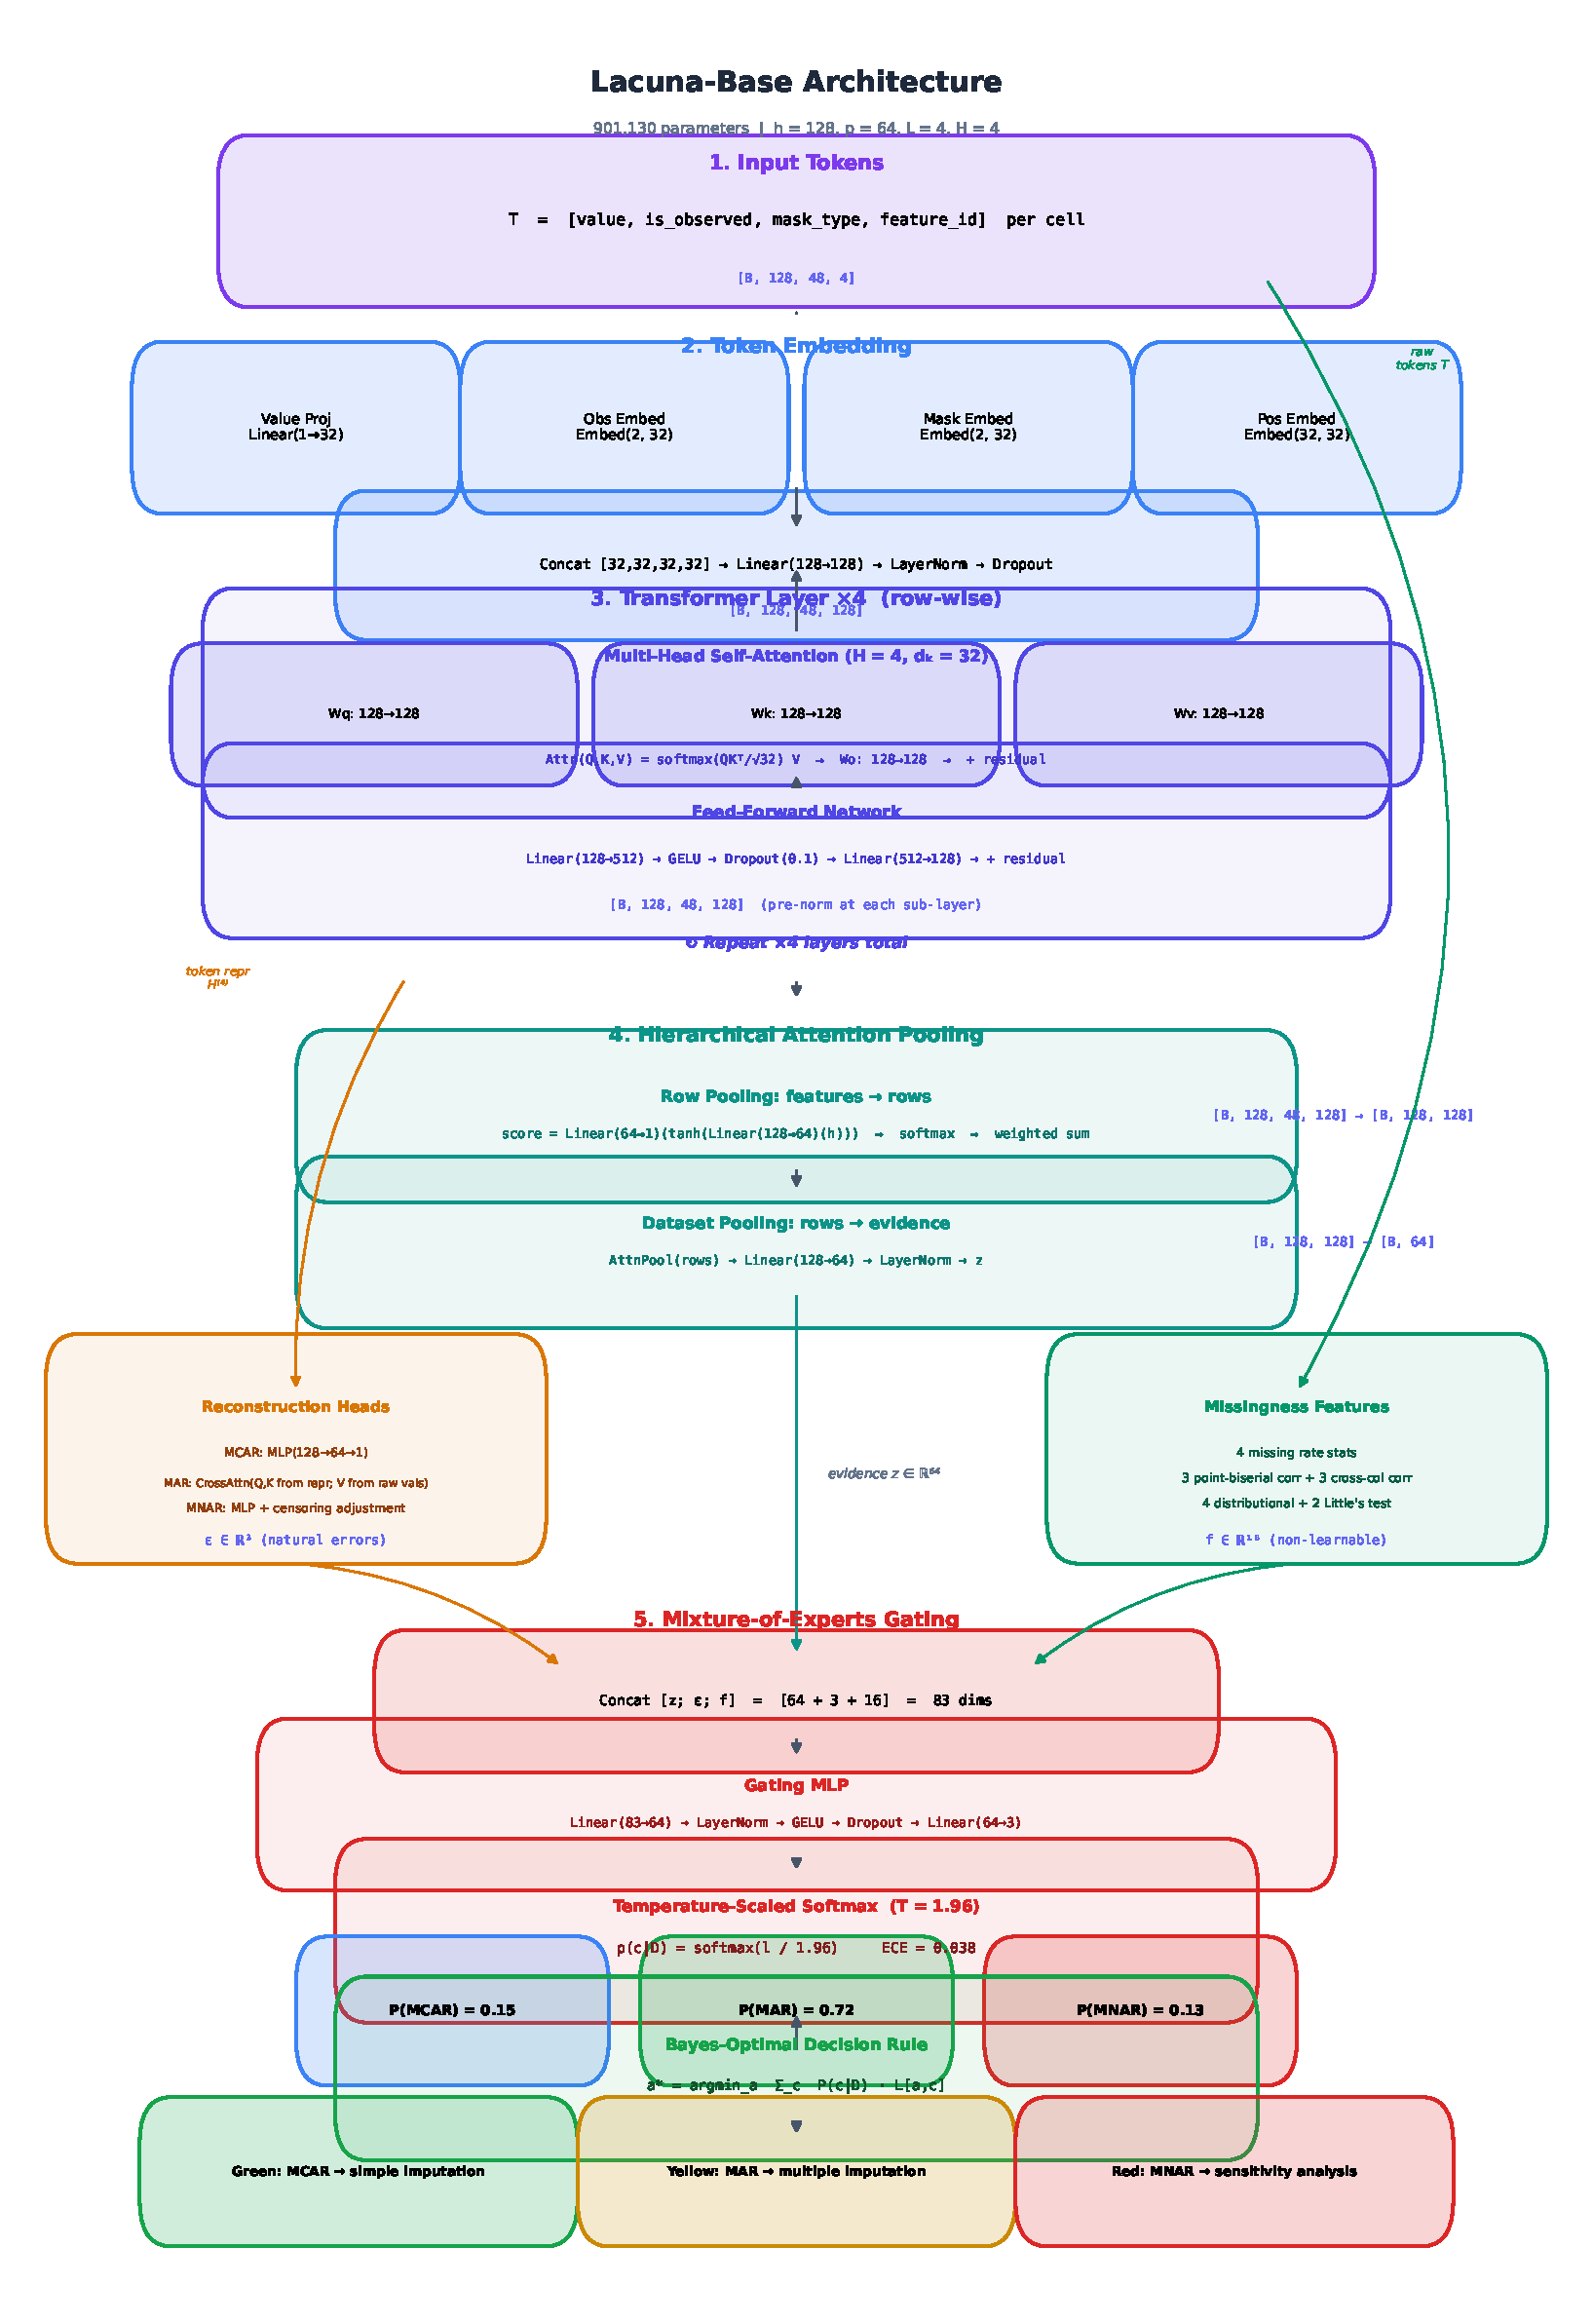
\includegraphics[width=\textwidth]{lacuna_architecture_diagram.pdf}
\caption{Complete \lacuna{}-Base architecture diagram showing the five-stage pipeline: (1)~token embedding, (2)~transformer encoder with row-wise attention, (3)~hierarchical pooling, (4)~reconstruction heads and missingness feature extraction, and (5)~MoE gating with Bayes-optimal decision. Tensor shapes are annotated at each stage. The base model uses hidden dimension $h = 128$, evidence dimension $p = 64$, $L = 4$ transformer layers, and $H = 4$ attention heads.}
\label{fig:architecture}
\end{figure}

\begin{figure}[p]
\centering
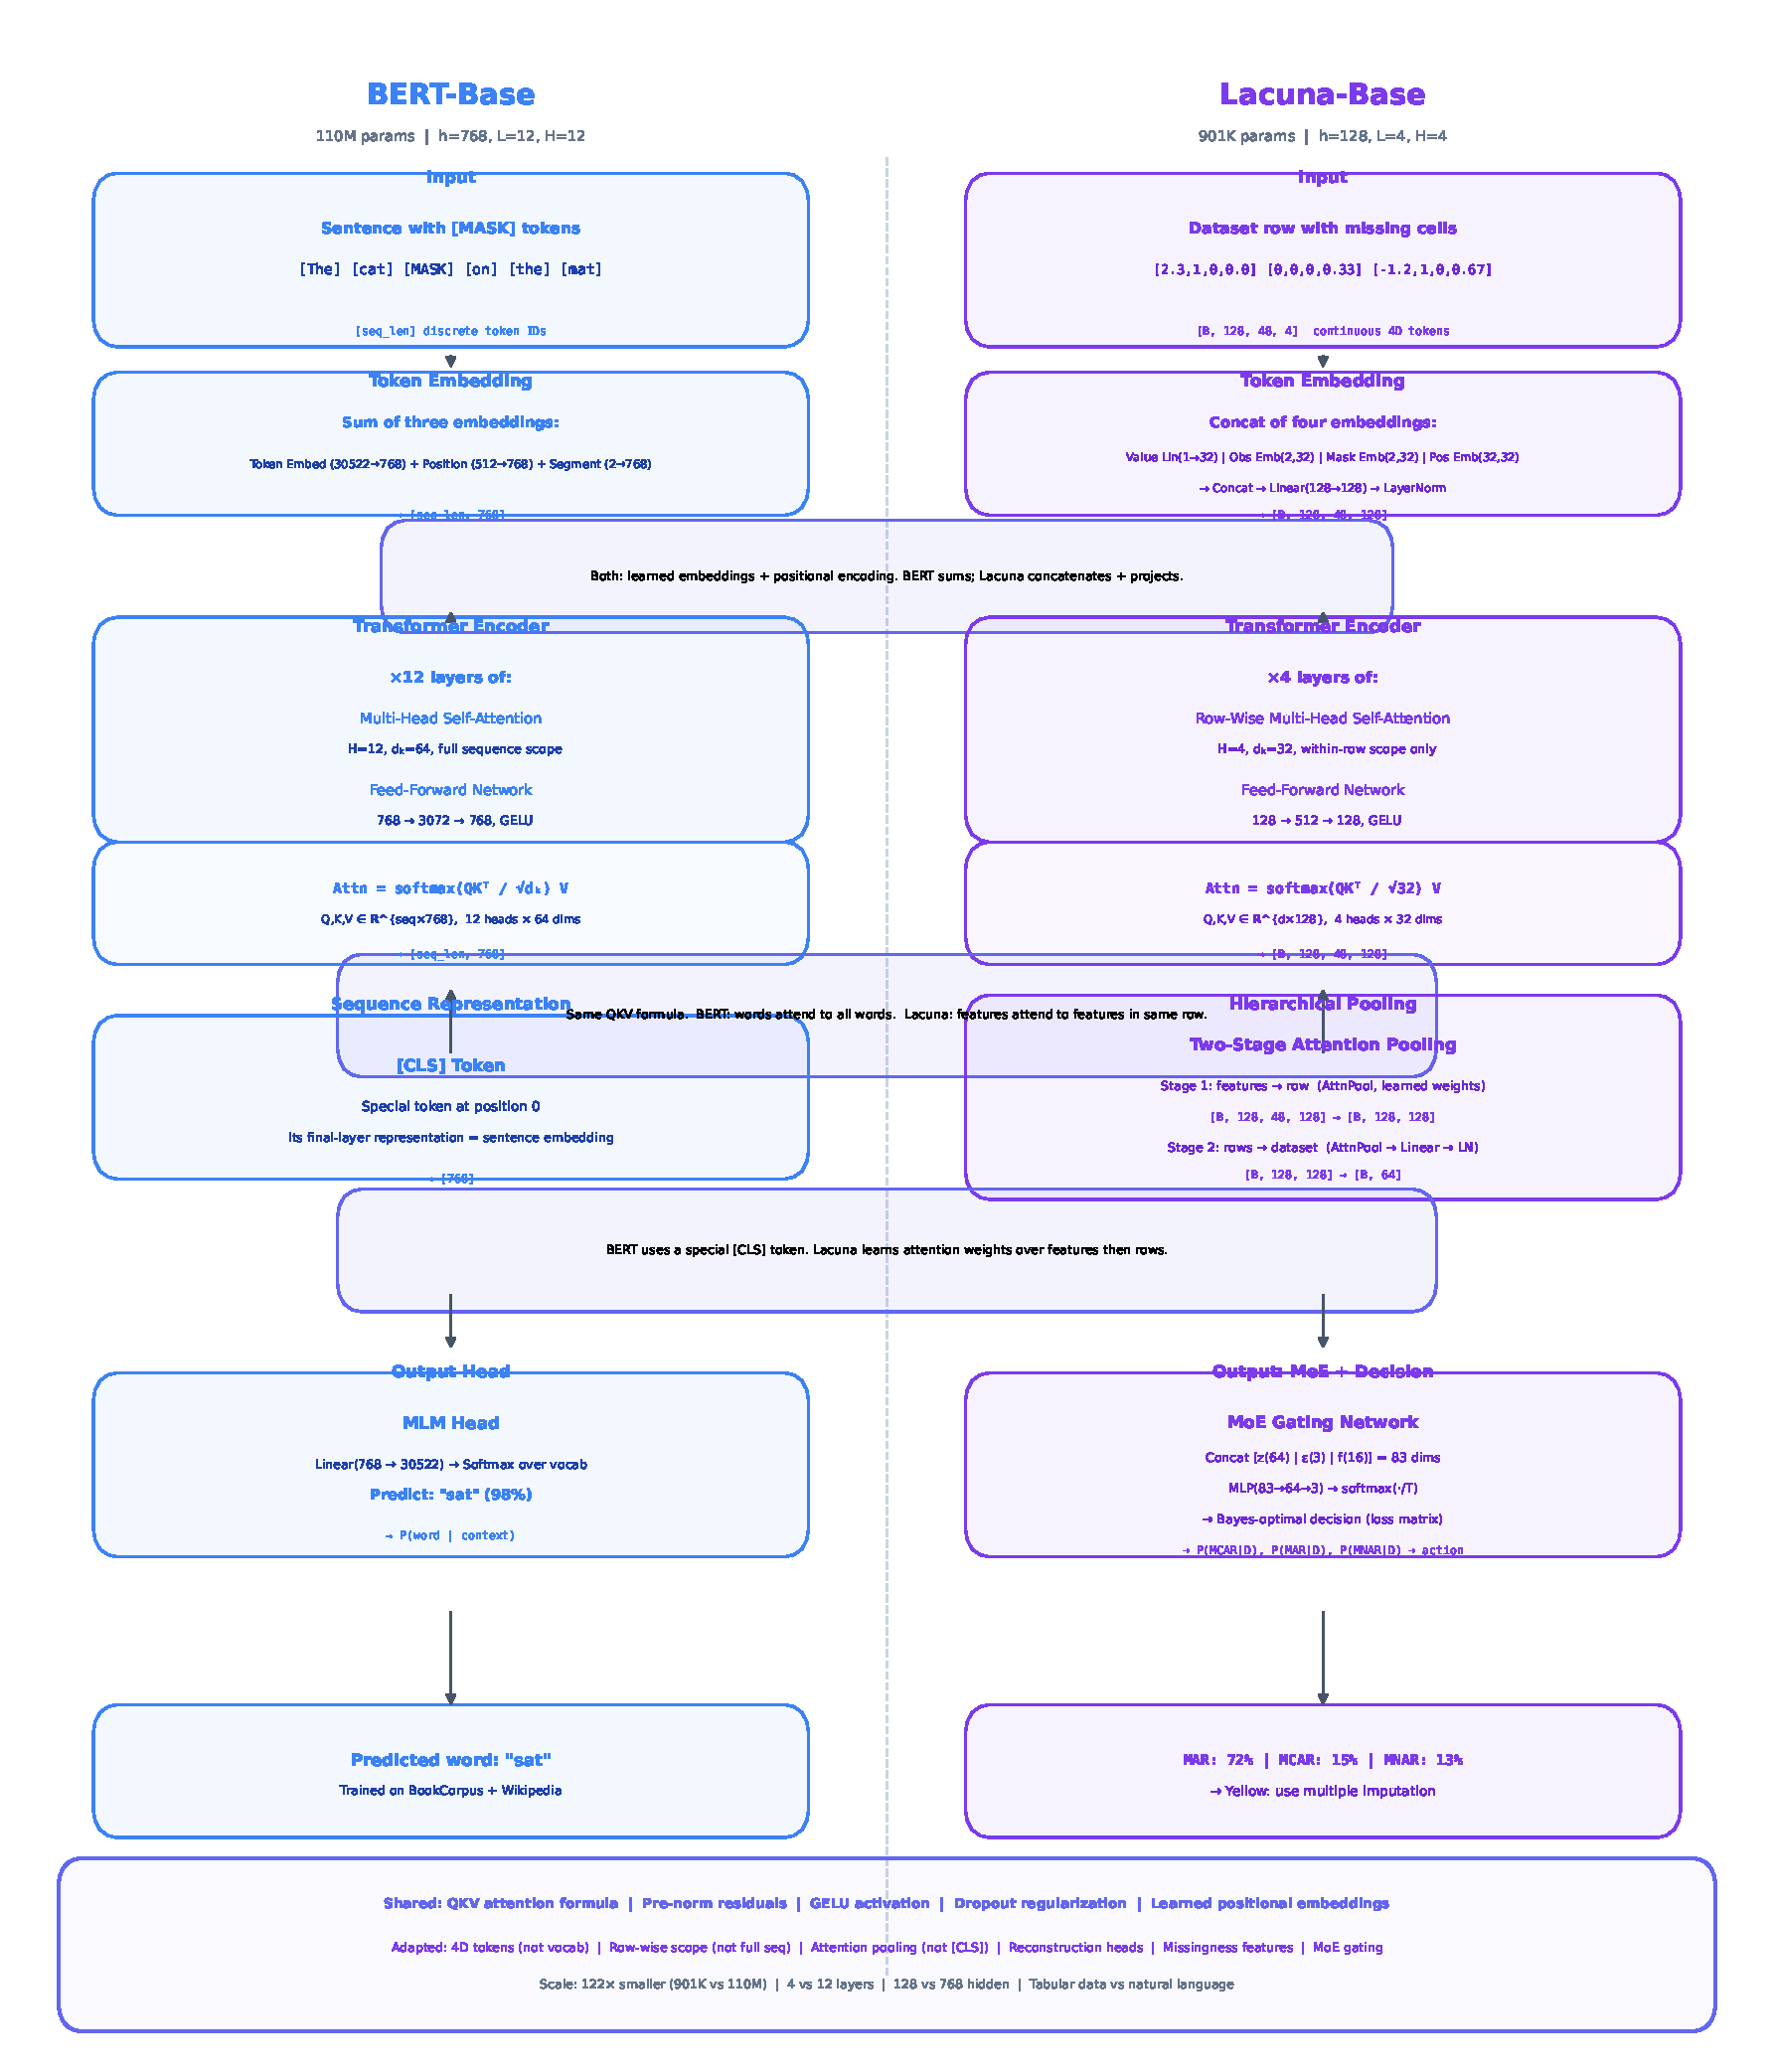
\includegraphics[width=\textwidth]{bert_lacuna_comparison.pdf}
\caption{Side-by-side architectural comparison of BERT-Base and \lacuna{}-Base. Shared design elements (blue shading) include bidirectional self-attention, pre-norm transformer layers, and residual connections. Key adaptations for the tabular domain (purple shading) include 4D cell tokens, row-wise attention scope, hierarchical attention pooling, and mechanism-specific reconstruction heads. \lacuna{} is approximately 122$\times$ smaller than BERT-Base (901K vs.\ 110M parameters) while sharing the same fundamental transformer architecture.}
\label{fig:comparison}
\end{figure}

% =====================================================================
\begin{thebibliography}{9}
\bibitem{devlin2019bert}
J.~Devlin, M.-W.~Chang, K.~Lee, and K.~Toutanova.
\newblock BERT: Pre-training of Deep Bidirectional Transformers for Language Understanding.
\newblock In \emph{NAACL-HLT}, 2019.
\end{thebibliography}

\end{document}
